\chapter{Resultados}
\label{chap:resultados}

Este capítulo apresenta os resultados experimentais do HoTHP em dois contextos: dados sintéticos, onde o processo gerador é conhecido, e dados reais, onde não é. Em seguida, visualizamos as intensidades aprendidas pelos modelos para entender o comportamento do viés de recência na prática, e realizamos uma ablação para isolar o efeito da escala temporal.

\section{Dados sintéticos}
\label{sec:resultados-sinteticos}

Os experimentos sintéticos seguem o protocolo descrito na Seção~\ref{sec:configuracao-experimental}, usando processos de Hawkes com kernel exponencial nos cenários de decaimento lento ($\beta$ pequeno) e rápido ($\beta$ grande). A Tabela~\ref{tab:resultados-sinteticos} resume os resultados para o protocolo \textit{train short, test long}, variando o comprimento de treinamento $L$ e o fator de extrapolação. A Figura~\ref{fig:extrapolacao-sintetica} visualiza a evolução da NLL em função de $\alpha$.

\begin{table}[h!]
\centering
\caption{NLL (média $\pm$ desvio padrão, 5 sementes) nos dados sintéticos. Valores menores indicam melhor desempenho. O melhor resultado para cada configuração está em negrito.}
\label{tab:resultados-sinteticos}
\begin{tabular}{llcccc}
\toprule
Cenário & Modelo & $1\times$ & $2\times$ & $5\times$ & $10\times$ \\
\midrule
\multirow{2}{*}{Decaimento lento} & RoTHP & $1{,}507 \pm 0{,}019$ & $2{,}016 \pm 0{,}236$ & $2{,}783 \pm 0{,}562$ & --- \\
                                   & HoTHP & $\mathbf{1{,}566 \pm 0{,}045}$ & $\mathbf{1{,}634 \pm 0{,}090}$ & $\mathbf{1{,}963 \pm 0{,}293}$ & --- \\
\midrule
\multirow{2}{*}{Decaimento rápido} & RoTHP & $\mathbf{1{,}681 \pm 0{,}005}$ & $1{,}942 \pm 0{,}153$ & $2{,}018 \pm 0{,}296$ & --- \\
                                    & HoTHP & $1{,}689 \pm 0{,}010$ & $\mathbf{1{,}702 \pm 0{,}015}$ & $\mathbf{1{,}750 \pm 0{,}059}$ & --- \\
\bottomrule
\end{tabular}
\end{table}

\begin{figure}[h!]
    \centering
    \captionsetup{width=14cm}
    \Caption{\label{fig:extrapolacao-sintetica} NLL (média $\pm$ desvio padrão, 5 sementes) em função do fator de extrapolação $\alpha$ nos cenários sintéticos. O HoTHP mantém a NLL estável à medida que $\alpha$ cresce, enquanto o RoTHP degrada progressivamente, especialmente no cenário de decaimento lento.}
    \UFCfig{}{
        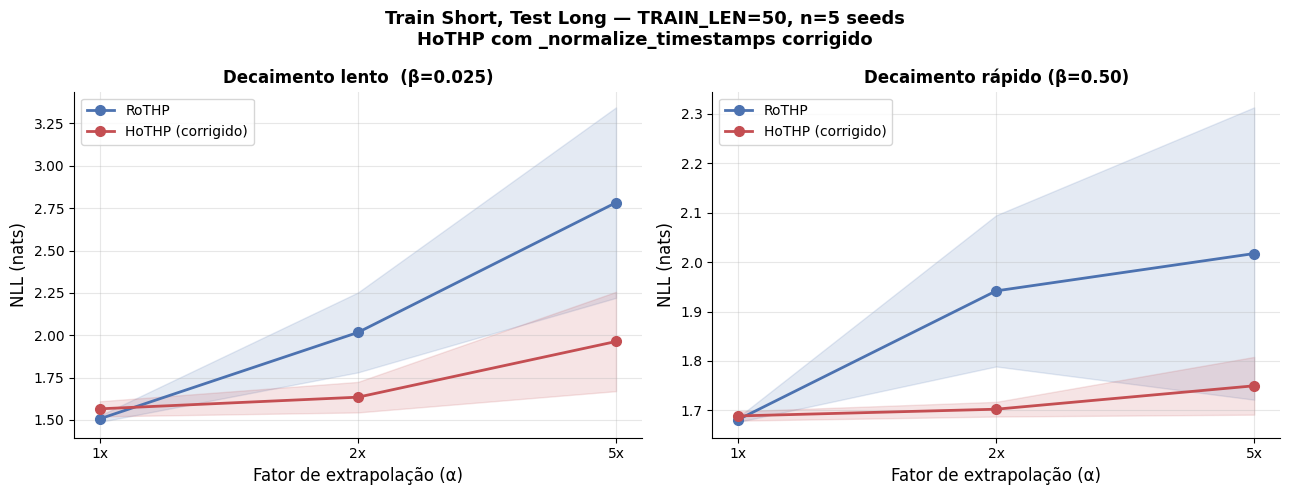
\includegraphics[width=14cm]{figuras/fig_extrapolation_nll_sintetico.png}
    }{
    }
\end{figure}

Nos dois cenários, o HoTHP mantém a NLL estável à medida que o fator de extrapolação cresce, enquanto o RoTHP apresenta degradação progressiva. Esse resultado é esperado: como o processo gerador possui kernel exponencial, o viés de recência do HoTHP está perfeitamente alinhado com a estrutura real dos dados. Para distâncias temporais não vistas no treino, o kernel hiperbólico continua a decair monotonicamente, enquanto o kernel trigonométrico do RoTHP oscila em fases não aprendidas.

\section{Dados reais}
\label{sec:resultados-reais}

Para avaliar o HoTHP em cenários mais realistas, realizamos experimentos em quatro datasets públicos de processos pontuais. A Tabela~\ref{tab:datasets-reais} descreve cada dataset.

\begin{table}[h!]
\centering
\caption{Datasets reais utilizados nos experimentos. $L_{\text{treino}}$ é o comprimento máximo de treinamento (número de eventos) e $L_{5\times}$ é o comprimento de teste na condição de extrapolação.}
\label{tab:datasets-reais}
\begin{tabular}{lccccc}
\toprule
Dataset & Tipos & Sequências (treino) & $L_{\text{treino}}$ & $L_{5\times}$ & Domínio \\
\midrule
Amazon         & 16 & 6.454  & 18 & 90  & Reviews de produtos \\
Stackoverflow  & 22 & 1.401  & 20 & 100 & Badges de usuários \\
Taxi           &  ?  & 1.400  &  7 & 38  & Corridas de táxi \\
Retweet        &  3 & 20.000 & 50 & 250 & Cascatas de retweets \\
\bottomrule
\end{tabular}
\end{table}

Seguimos o mesmo protocolo \textit{train short, test long}: treinamos cada modelo com sequências truncadas em $L_{\text{treino}}$ eventos e avaliamos tanto no comprimento de treino ($1\times$) quanto na extrapolação ($5\times$). Usamos três sementes (2019, 2020, 2021), 100 épocas e os mesmos hiperparâmetros da Seção~\ref{subsec:modelos-comparados}. Para o Amazon e Stackoverflow, comparamos THP, RoTHP e HoTHP; para o Taxi e Retweet, comparamos apenas RoTHP e HoTHP.

A Tabela~\ref{tab:resultados-reais} apresenta os resultados.

\begin{table}[h!]
\centering
\caption{NLL nos datasets reais (média $\pm$ desvio padrão, 3 sementes). $\Delta$NLL é a diferença $5\times$ menos $1\times$: valores negativos indicam que o modelo melhora com sequências mais longas. Valores menores de NLL são melhores. O melhor resultado para cada dataset e condição está em negrito.}
\label{tab:resultados-reais}
\resizebox{\textwidth}{!}{%
\begin{tabular}{llcccc}
\toprule
Dataset & Modelo & NLL $1\times$ & NLL $5\times$ & $\Delta$NLL & Acc $5\times$ \\
\midrule
\multirow{3}{*}{Amazon}
    & THP    & $2{,}274 \pm 0{,}002$ & $2{,}244 \pm 0{,}007$ & $-0{,}030$ & $0{,}322 \pm 0{,}004$ \\
    & RoTHP  & $2{,}272 \pm 0{,}004$ & $2{,}252 \pm 0{,}002$ & $-0{,}020$ & $0{,}321 \pm 0{,}004$ \\
    & HoTHP  & $2{,}268 \pm 0{,}002$ & $\mathbf{2{,}194 \pm 0{,}002}$ & $\mathbf{-0{,}074}$ & $\mathbf{0{,}340 \pm 0{,}002}$ \\
\midrule
\multirow{3}{*}{Stackoverflow}
    & THP    & $2{,}745 \pm 0{,}011$ & $\mathbf{2{,}521 \pm 0{,}020}$ & $-0{,}224$ & $0{,}451 \pm 0{,}002$ \\
    & RoTHP  & $2{,}753 \pm 0{,}005$ & $2{,}538 \pm 0{,}003$ & $-0{,}215$ & $0{,}450 \pm 0{,}000$ \\
    & HoTHP  & $2{,}742 \pm 0{,}020$ & $2{,}530 \pm 0{,}023$ & $-0{,}212$ & $0{,}451 \pm 0{,}003$ \\
\midrule
\multirow{2}{*}{Taxi}
    & RoTHP  & $-0{,}269 \pm 0{,}005$ & $-0{,}176 \pm 0{,}041$ & $+0{,}092$ & $0{,}907 \pm 0{,}002$ \\
    & HoTHP  & $-0{,}271 \pm 0{,}006$ & $\mathbf{-0{,}212 \pm 0{,}009}$ & $\mathbf{+0{,}059}$ & $0{,}907 \pm 0{,}003$ \\
\midrule
\multirow{2}{*}{Retweet}
    & RoTHP  & $12{,}5 \pm 4{,}9$ & $\mathbf{121 \times 10^3}$ & --- & $0{,}520 \pm 0{,}042$ \\
    & HoTHP  & $12{,}5 \pm 4{,}8$ & $367 \times 10^3$ & --- & $0{,}518 \pm 0{,}039$ \\
\bottomrule
\end{tabular}
}
\end{table}

Três padrões distintos emergem dos resultados:

\textbf{Amazon: HoTHP vence.} O HoTHP obtém a melhor NLL em ambas as condições e apresenta o maior ganho na extrapolação ($\Delta\text{NLL} = -0{,}074$, contra $-0{,}020$ do RoTHP). A diferença é pequena em valor absoluto, mas consistente entre as três sementes (desvio padrão de $0{,}002$).

\textbf{Stackoverflow: empate.} Os três modelos apresentam NLL praticamente idênticas em $5\times$, com diferenças dentro da margem de erro. Nenhum modelo se beneficia mais do que os outros com sequências mais longas. Isso sugere que o dataset não possui estrutura temporal que diferencie os vieses posicionais dos três modelos.

\textbf{Taxi: empate com leve vantagem do HoTHP.} O HoTHP degrada menos na extrapolação ($\Delta\text{NLL} = +0{,}059$ contra $+0{,}092$ do RoTHP), mas a diferença é modesta e a variância do RoTHP é alta.

\textbf{Retweet: ambos os modelos falham.} A NLL em $5\times$ explode para valores na ordem de $10^5$, com o HoTHP pior que o RoTHP ($367 \times 10^3$ contra $121 \times 10^3$). A escala temporal extrema desse dataset (intervalos entre eventos de até 582.928 unidades de tempo) faz com que o kernel hiperbólico sature numericamente, como discutido na Seção~\ref{sec:estabilidade-numerica}.

\subsection{Convergência do treinamento}
\label{subsec:convergencia}

A Figura~\ref{fig:convergencia} mostra as curvas de convergência da NLL de validação ao longo das 100 épocas de treinamento. Nos datasets Amazon e Stackoverflow, os três modelos convergem de forma suave, com a NLL estabilizando após a época 50. No Amazon, a curva ainda apresenta uma tendência de queda suave nas últimas 20 épocas, mas com declive inferior a $0{,}01$ por época, o que indica que épocas adicionais beneficiariam todos os modelos igualmente sem alterar o ranking.

No Taxi, o RoTHP apresenta maior variância entre sementes nas épocas iniciais (10 a 40), mas converge para o mesmo patamar que o HoTHP após a época 40. No Retweet, a convergência revela o colapso numérico: 2 de 3 sementes estabilizam em NLL $\approx 15{,}9$, enquanto apenas uma semente (2019) converge para valores informativos ($\text{NLL} \approx 5{,}5$). A banda de desvio padrão resultante é enorme, confirmando visualmente a instabilidade reportada na Tabela~\ref{tab:resultados-reais}.

\begin{figure}[h!]
    \centering
    \captionsetup{width=14cm}
    \Caption{\label{fig:convergencia} Curvas de convergência da NLL de validação (média $\pm$ desvio padrão, 3 sementes). As primeiras épocas foram omitidas para melhorar a visualização. No Amazon e Stackoverflow, todos os modelos convergem de forma suave. No Taxi, o RoTHP é mais instável nas épocas iniciais. No Retweet, a banda larga do RoTHP reflete o colapso de 2 das 3 sementes.}
    \UFCfig{}{
        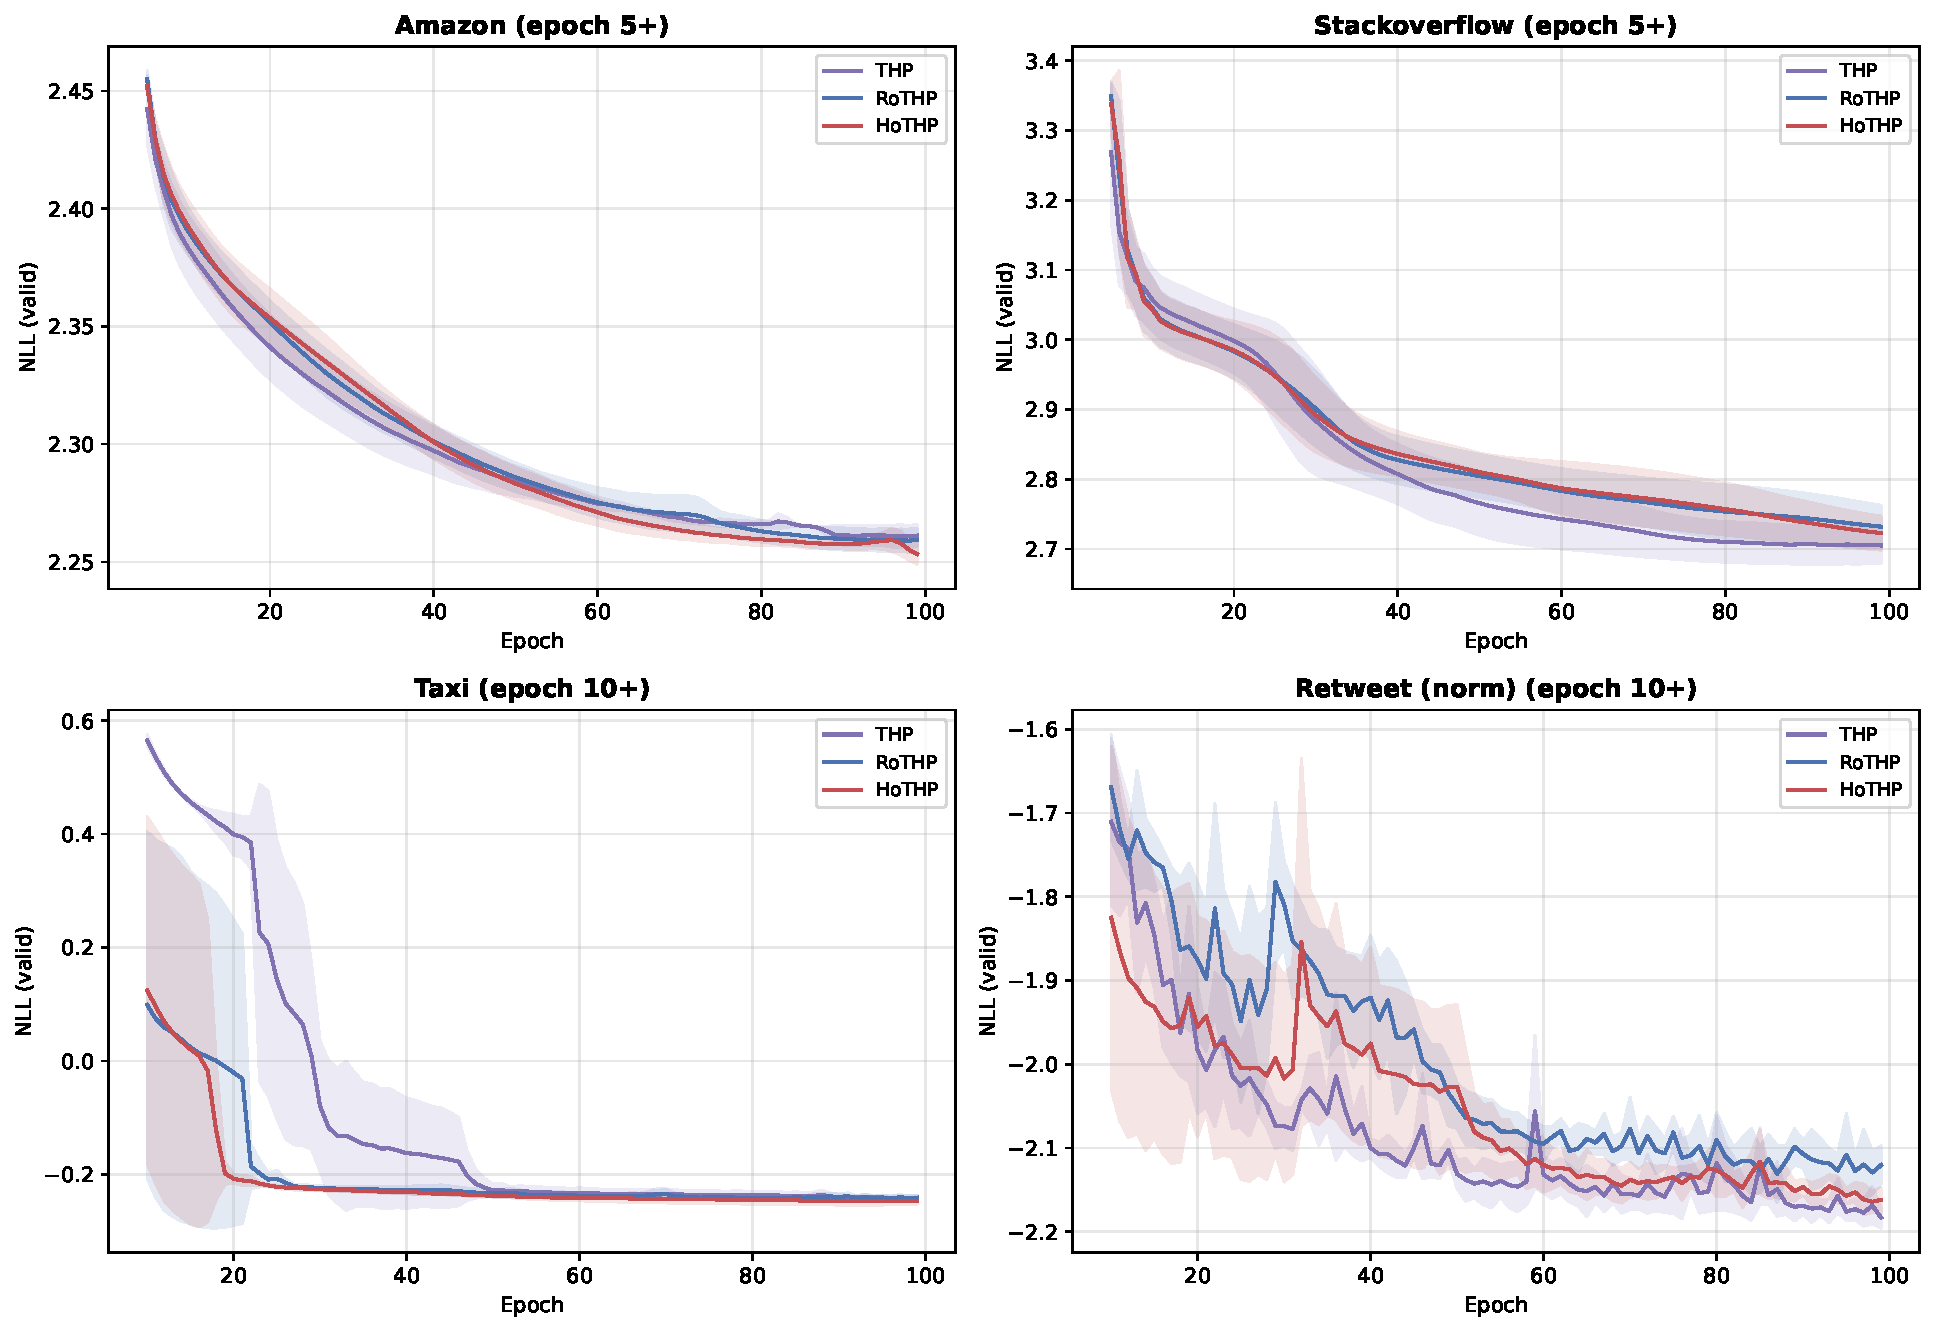
\includegraphics[width=14cm]{figuras/fig_convergencia.pdf}
    }{
    }
\end{figure}

\section{Intensidades aprendidas pelos modelos}
\label{sec:intensidades-aprendidas}

Para entender por que o HoTHP se comporta de forma diferente em cada dataset, extraímos a função de intensidade condicional $\lambda^*(t)$ que cada modelo treinado calcula para sequências de teste representativas. A Figura~\ref{fig:intensidades} mostra a intensidade total $\lambda^*(t) = \sum_k \lambda_k^*(t)$ ao longo do tempo para os datasets Amazon, Stackoverflow e Retweet.

\begin{figure}[h!]
    \centering
    \captionsetup{width=14cm}
    \Caption{\label{fig:intensidades} Intensidade condicional $\lambda^*(t)$ aprendida pelo THP (laranja), RoTHP (azul) e HoTHP (verde) para uma sequência de teste de cada dataset. As barras verticais cinzas indicam os eventos. No Amazon, a intensidade cresce entre eventos e cai ao ocorrer um evento (auto-inibição). No Stackoverflow, a intensidade é aproximadamente constante (processo sem memória). No Retweet, ambos os modelos colapsam para $\lambda^* \approx 0$ após o burst inicial devido à escala temporal extrema.}
    \UFCfig{}{
        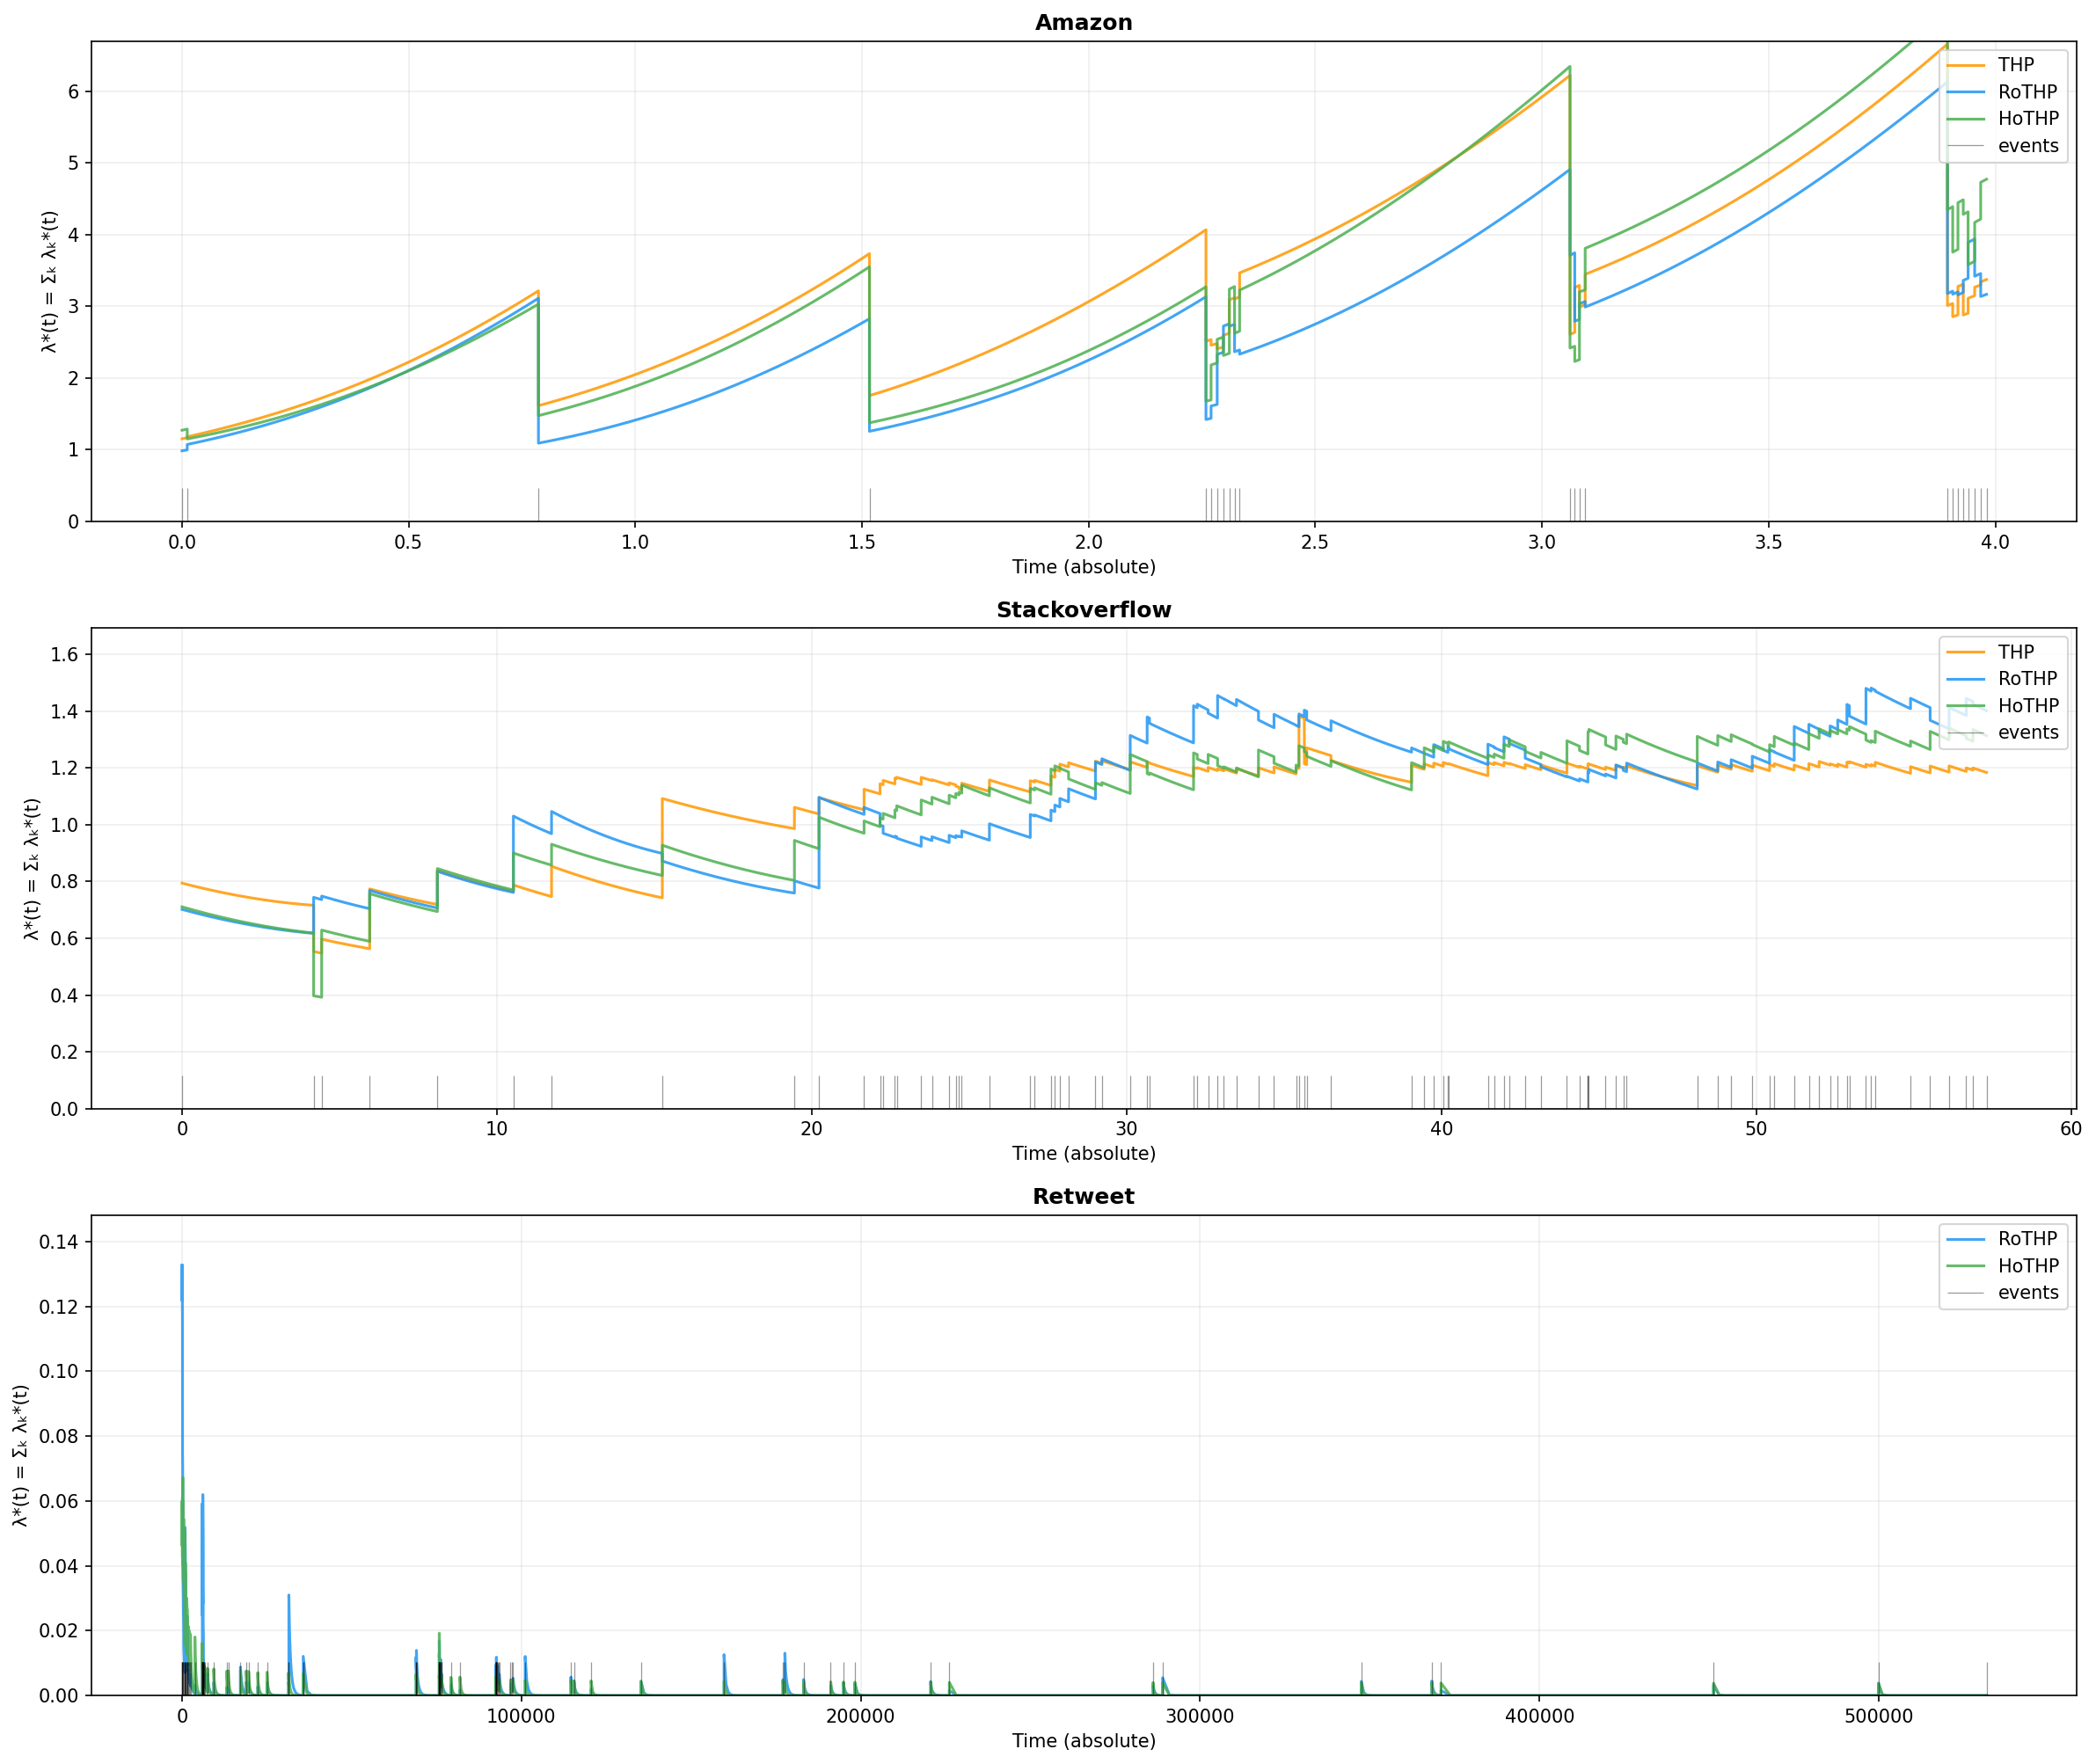
\includegraphics[width=14cm]{figuras/fig_model_intensity.png}
    }{
    }
\end{figure}

No Amazon, a intensidade cresce entre eventos e cai quando um evento ocorre, indicando que cada evento reduz a chance de novos eventos no curto prazo. Mesmo assim, o evento mais recente é o mais informativo para a previsão, o que explica por que o viés de recência do HoTHP ajuda nesse dataset. No Stackoverflow, os três modelos aprendem uma intensidade praticamente plana, sem reação visível aos eventos, caracteristico de um processo com pouca memória temporal, e nenhum viés posicional consegue se diferenciar. No Retweet, os modelos só reagem ao burst inicial e depois a intensidade cai para praticamente zero, porque os intervalos entre eventos são grandes demais para qualquer função de decaimento.

A observação do Amazon é particularmente relevante à luz da Seção~\ref{sec:onde-atua-vies}: o HoTHP vence nesse dataset apesar de o processo ser auto-inibitório, não auto-excitante. Isso confirma que o viés de recência atua na atenção (``quais eventos passados são mais relevantes'') e não na intensidade (``a intensidade sobe ou desce após um evento''). No Amazon, o evento mais recente é o mais informativo para prever o próximo e o decaimento exponencial na atenção captura isso corretamente.

\section{Ablação: normalização temporal do Retweet}
\label{sec:ablacao-retweet}

O colapso numérico observado no Retweet levanta uma questão: o problema é a escala temporal ou o próprio viés do HoTHP? Para isolar esses fatores, realizamos uma ablação em que normalizamos os timestamps do Retweet antes do treinamento.

A normalização consiste em dividir todos os instantes de cada sequência pela média dos intervalos daquela sequência:
%
\begin{equation}
    \tilde{t}_i = \frac{t_i - t_1}{\bar{\Delta t}}, \quad \text{onde} \quad \bar{\Delta t} = \frac{1}{N-1} \sum_{i=2}^{N} (t_i - t_{i-1}).
    \label{eq:normalizacao-retweet}
\end{equation}
%
Após essa operação, o intervalo médio entre eventos passa a ser aproximadamente~1 em todas as sequências, com o intervalo máximo reduzido de~582.928 para aproximadamente~227. A estrutura temporal (ordem dos eventos, padrões de clustering, tipos) é preservada; apenas a escala numérica muda.

Treinamos o RoTHP e o HoTHP no Retweet normalizado com os mesmos hiperparâmetros (3 sementes, 100 épocas, $L_{\text{treino}} = 50$, $L_{5\times} = 250$) e comparamos com os resultados originais.

\begin{table}[h!]
\centering
\caption{Ablação: efeito da normalização temporal no Retweet. ``Original'' usa os timestamps brutos; ``Normalizado'' usa os timestamps divididos pela média dos gaps. Média $\pm$ desvio padrão (3 sementes).}
\label{tab:ablacao-retweet}
\begin{tabular}{llcccc}
\toprule
Versão & Modelo & NLL $1\times$ & NLL $5\times$ & Acc $1\times$ & Acc $5\times$ \\
\midrule
\multirow{2}{*}{Original}
    & RoTHP  & $12{,}456 \pm 6{,}038$ & $1 \times 10^{5}$ & $0{,}496 \pm 0{,}072$ & $0{,}520 \pm 0{,}051$ \\
    & HoTHP  & $12{,}517 \pm 5{,}932$ & $4 \times 10^{5}$ & $0{,}495 \pm 0{,}071$ & $0{,}518 \pm 0{,}047$ \\
\midrule
\multirow{2}{*}{Normalizado}
    & RoTHP  & $-2{,}197 \pm 0{,}163$ & $88{,}856 \pm 144{,}800$ & $0{,}588 \pm 0{,}036$ & $0{,}562 \pm 0{,}014$ \\
    & HoTHP  & $-2{,}168 \pm 0{,}010$ & $\mathbf{-0{,}542 \pm 0{,}004}$ & $0{,}591 \pm 0{,}002$ & $\mathbf{0{,}588 \pm 0{,}004}$ \\
\bottomrule
\end{tabular}
\end{table}

A normalização resolve o colapso numérico de forma inequívoca. Com timestamps brutos, a NLL em $1\times$ é de aproximadamente $12{,}5$ para ambos os modelos e a NLL em $5\times$ explode para a ordem de $10^5$. Com timestamps normalizados, a NLL em $1\times$ cai para valores negativos e o treino converge em todas as sementes.

A diferença entre os modelos aparece na extrapolação. O HoTHP normalizado obtém NLL $5\times = -0{,}542 \pm 0{,}004$, praticamente invariante entre sementes. O RoTHP normalizado, embora muito melhor que a versão com dados brutos, ainda é instável. Uma das sementes atinge NLL $5\times = 255{,}9$, resultando numa média de $88{,}9 \pm 144{,}8$. A acurácia de tipos segue o mesmo padrão: o HoTHP normalizado mantém Acc $5\times = 0{,}588$ com desvio de $0{,}004$, enquanto o RoTHP cai para $0{,}562$.

Esses resultados permitem separar os dois fatores que prejudicam o desempenho no Retweet. O problema primário era a escala numérica. A normalização beneficia ambos os modelos drasticamente. Mas mesmo com a escala corrigida, o HoTHP supera o RoTHP na extrapolação, confirmando que o viés de recência é vantajoso nesse dataset quando a escala temporal permite sua calibração. A instabilidade residual do RoTHP (com uma semente ainda explodindo em $5\times$) reforça a fragilidade do kernel oscilatório na extrapolação, observada também nos dados sintéticos.

\section{Discussão}
\label{sec:discussao-resultados}

Os resultados em dados reais mostram que o viés de recência do HoTHP é benéfico em alguns cenários e neutro ou prejudicial em outros. A análise das intensidades aprendidas sugere que o fator determinante não é se o processo é auto-excitante ou auto-inibitório, mas sim se os eventos recentes são mais informativos do que os distantes para a construção do estado oculto.

No Amazon, onde o HoTHP obtém o melhor resultado, o processo é auto-inibitório: a intensidade cresce com o tempo desde o último evento. Mesmo assim, o viés de recência ajuda, porque o evento imediatamente anterior é o mais relevante para prever o próximo. O decaimento exponencial na atenção captura corretamente essa relação de relevância decrescente.

No Stackoverflow, onde os três modelos empatam, a intensidade é praticamente constante. Isso indica um processo com pouca ou nenhuma memória temporal, no qual todos os eventos passados são igualmente (pouco) informativos. O viés de recência do HoTHP não prejudica significativamente (a intensidade constante mostra que o modelo consegue compensar na camada de intensidade), mas também não ajuda, porque não há estrutura temporal para explorar.

No Retweet, o problema é duplo: a escala temporal extrema causa colapso numérico, e a estrutura de cascatas virais pode não se alinhar com o decaimento exponencial. A ablação da Seção~\ref{sec:ablacao-retweet} separou esses dois fatores e mostrou que o problema primário era a escala: com normalização, o HoTHP obtém o melhor resultado de todo o benchmark (NLL $5\times = -0{,}542$), com variância quase zero entre sementes. O RoTHP, mesmo com normalização, ainda apresenta instabilidade na extrapolação, com uma semente atingindo NLL $= 255{,}9$.

O HoTHP se mostra mais eficaz quando duas condições são satisfeitas simultaneamente: (i) o processo possui memória temporal de curto alcance, de modo que eventos recentes são mais informativos que distantes; e (ii) a escala dos intervalos entre eventos permite que o parâmetro $\theta'$ seja calibrado adequadamente durante o treinamento, sem saturação numérica. A ablação do Retweet confirma que a condição (ii) pode ser resolvida por pré-processamento, e quando o é, o viés de recência do HoTHP se mostra consistentemente vantajoso.

\subsection{Custo computacional versus benefício na extrapolação}
\label{subsec:custo-beneficio}

O kernel hiperbólico do HoTHP envolve mais operações que o kernel trigonométrico do RoTHP, o que se reflete no tempo de treinamento. A Tabela~\ref{tab:tempo-treino} apresenta os tempos médios de treinamento (100 épocas, 3 sementes) para cada combinação de dataset e modelo.

\begin{table}[h!]
\centering
\caption{Tempo médio de treinamento (minutos, 3 sementes). O fator indica quantas vezes o HoTHP é mais lento que o RoTHP.}
\label{tab:tempo-treino}
\begin{tabular}{lccc}
\toprule
Dataset & RoTHP (min) & HoTHP (min) & Fator \\
\midrule
Stackoverflow  &  2,4 &  3,1 & $1{,}26\times$ \\
Amazon         &  9,4 & 11,8 & $1{,}25\times$ \\
Taxi           &  1,9 &  2,0 & $1{,}05\times$ \\
Retweet (norm) & 43,5 & 97,6 & $2{,}24\times$ \\
\bottomrule
\end{tabular}
\end{table}

O overhead varia de $1{,}05\times$ (Taxi) a $2{,}24\times$ (Retweet normalizado), sendo mais pronunciado em datasets com sequências longas, onde o cálculo do kernel hiperbólico domina o tempo por batch. Para datasets de comprimento moderado (Stackoverflow, Amazon, Taxi), o custo adicional é inferior a $25\%$.

Esse custo, contudo, é pago uma única vez durante o treinamento. Na inferência, o modelo treinado é aplicado a sequências potencialmente muito mais longas do que as vistas no treino --- exatamente o cenário de extrapolação. Nesse contexto, o que importa não é a velocidade do treinamento, mas se o modelo produz resultados válidos. Os resultados da Tabela~\ref{tab:ablacao-retweet} ilustram o ponto de forma clara: no Retweet normalizado com extrapolação $5\times$, o RoTHP obtém NLL $= 88{,}9 \pm 144{,}8$ (com uma semente explodindo para $255{,}9$), enquanto o HoTHP obtém NLL $= -0{,}542 \pm 0{,}004$. Treinar o RoTHP $2{,}2\times$ mais rápido para depois obter resultados inutilizáveis na extrapolação não constitui uma vantagem prática.
